% $Id$
% ---------------------------------------------------------------------------
%
% Copyright (c) 2008 Interlegis
%
% This is part of the relatorio-modelo.
%
% relatorio-modelo is free software; you can redistribute it and/or
% modify it under the terms of the GNU General Public License as
% published by the Free Software Foundation; either version 3 of the
% License, or (at your option) any later version.
%
% relatorio-modelo is distributed in the hope that it will be useful,
% but WITHOUT ANY WARRANTY; without even the implied warranty of
% MERCHANTABILITY or FITNESS FOR A PARTICULAR PURPOSE. See the GNU
% General Public License for more details.
%
% You should have received a copy of the GNU General Public License
% along with this program; see the file COPYING.  If not, see
% <http://www.gnu.org/licenses/>.
%

\documentclass[a4paper,12pt]{article}
\textheight 22.5cm
\usepackage[brazil]{babel}      % suporte ao portugues brasil
\usepackage[utf8]{inputenc}     % Codificacao dos caracteres (use a
                                % codificacao latin1 caso seu
                                % sistema/editor nao suporte utf8).
\usepackage[T1]{fontenc}
\usepackage{indentfirst}        % indenta o primeiro paragrafo 
\usepackage{graphicx}           % uso para imagens
\usepackage{dsfont}             % fonte

\usepackage{fancyhdr}           % permite alterar o cabecalho
\pagestyle{fancy}               % configura o estilo padrao

\newcommand{\titulo}{Produto: Webscan}
\newcommand{\subtitulo}{Relatório III}
\newcommand{\subsubtitulo}{Manual de instruções. Documentos de ajuda sensitiva ao contexto integrado às várias telas do sistema}
\newcommand{\autor}{Sérgio Oliveira Campos}
\newcommand{\numcontrato}{2008/000514} % Número do contrato caso seja consultor.
                % novos comandos

\usepackage[pdftex,%            % formatacao no PDF
pdfauthor={\autor},%
pdftitle={\titulo - \subtitulo},%
]{hyperref}
\hypersetup{backref=true,pdfpagemode=UseOutlines,colorlinks=true,
  breaklinks=true,hyperindex,linkcolor=blue,anchorcolor=black,
  citecolor=blue,filecolor=magenta,menucolor=red,pagecolor=red,
  urlcolor=cyan,bookmarks=true,bookmarksopen=true,pdfpagelayout=SinglePage,
  pdfpagetransition=Dissolve}


\begin{document}
% $Id$
% ---------------------------------------------------------------------------
%
%  This is part of the relatorio-modelo.
%  Copyright (C) 2008 Interlegis
%  See the file relatorio.tex for copying conditions.
%

\lhead {
  \begin{picture}(0,0) 
    
\includegraphics[scale=0.65]{imagens/cabecalho.pdf} 
  \end{picture} 
}
\chead{}
\rhead{}
\renewcommand{\headrulewidth}{0pt}

%
% Local variables:
%   mode: flyspell
%   TeX-master: "relatorio.tex"
% End:
%

% $Id$
% ---------------------------------------------------------------------------
%
%  This is part of the relatorio-modelo.
%  Copyright (C) 2008 Interlegis
%  See the file relatorio.tex for copying conditions.
%

\textsf{\vspace{6cm}}
\begin{center}
  \noindent
  \huge{
    \textbf{\titulo}
  } \\
  \Large{
    \textbf{\subtitulo}
  }\\
  \large{
    \textbf{\subsubtitulo}
  }

  \vspace{9cm}

  \large{
    \textbf{\autor}\\
    \textsf{Contrato N$^{\circ}$: \numcontrato}\\
  }
\end{center}
\cfoot{}                        % retira o rodape

%
% Local variables:
%   mode: flyspell
%   TeX-master: "relatorio.tex"
% End:
%


% configura o rodape do conteudo pre-textual para numeros romanos
\clearpage
\cfoot{\thepage}
\setcounter{page}{1}
\pagenumbering{Roman}

\tableofcontents
\listoffigures
\listoftables

% configura o rodape das paginas de conteudo para numeros convencionais
\clearpage
\setcounter{page}{1}
\pagenumbering{arabic}

% conteudo
\section{Introdução}
\label{sec:intro}

Na segunda fase do projeto {\it webscan} foi realizada a atividade de 
codificação. Para que esta etapa fosse realizada com sucesso algumas 
mudanças foram feitas na documentação apresentada no relatório I. 
Estas mudanças serão descritas neste relatório porém estarão mais detalhadas 
no relatório III.

Neste documento serão apresentados e descritos os principais pontos 
necessários para o entendimento do código fonte do produto, 
tais como estrutura de diretórios e algoritmos utilizados.

\section{Instalação}
\label{sec:instalacao}
Este capítulo descreve os passos para a instalação do módulo daemon do
{\it webscan}. O módulo UI não exige instalação e por esse motivo não

Estas instruções estão divididas em 2 seções que descrevem os
procedimentos de instalação nos sistemas Linux e Windows respectivamente.

Em ambos sistemas a instalação dos drivers específicos dos scanners que 
serão utilizados é necessária para que software trabalhe corretamente.

\subsection{Linux}
Esta seção cobre a instalação do produto {\it webscan} na distribuição
Ubuntu e outras que compartilham o mesmo tipo de gerenciamento de pacotes.

As linhas de comando apresentadas nesta seção poderão iniciar com `\#' ou
`\$'; quando iniciadas com `\#' significa que elas precisam ser executadas 
com super-usuário (ou root), caso contrário um usuário convencional será
suficiente.

\subsubsection{Pré-Requisitos}
Boa parte das dependências do {\it webscan} podem ser instaladas através 
do software apt-get executando-se o comando:

\begin{verbatim}
 # apt-get install [nome_do_pacote nome_de_outro_pacote]
\end{verbatim}

Os pacotes necessários são:

\begin{itemize}
    \item python
    \item python-imaging
    \item python-imaging-sane
    \item python-setuptools
    \item python-simplejson
\end{itemize}

Após instalados os pacotes do sistema operacional será necessária a 
instalação do Django. Baixe a versão 1.0 em:
\begin{verbatim}
http://www.djangoproject.com/
\end{verbatim}

Após baixar o pacote do Django a instalação deve ser realizada com as 
seguintes linhas de comando:
\begin{verbatim}
 $ tar xzvf Django-1.0.tar.gz
 $ cd Django-1.0
 # python setup.py install
\end{verbatim}

\subsubsection{Módulo daemon}
Para instalar o módulo daemon será necessário a cópia do 
código-fonte para o servidor onde o scanner será utilizado.

O código-fonte pode ser obtido no CD que segue junto a este
relatório. A versão atualizada deste código também pode ser encontrada
no repositório do projeto Interlegis em:
\begin{verbatim}
http://repositorio.interlegis.gov.br/digidoc/trunk/
\end{verbatim}
 

\subsection{Windows}

\section{Instruções de utilização}
\label{sec:utilizacao}

Para facilitar o entendimento da interface do {\it webscan} podemos
dividi-la em diferente elementos, como mostra a figura \ref{fig:interface}.

\begin{figure}[ht]
\begin{center}
\scalebox{0.55} {
    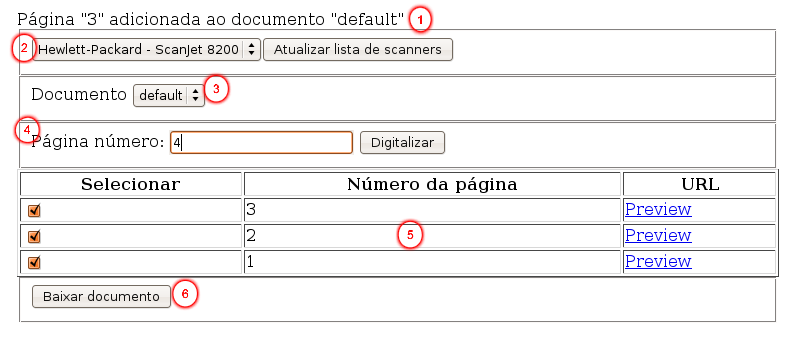
\includegraphics{imagens/interface.png}}
\end{center}
  \caption{Elementos da interface gráfica numerados}
  \label{fig:interface}
\end{figure}

A descrição de cada elemento e respectivas intruções de uso
serão apresentadas nas seções a seguir.


\subsection{Elemento 1: Área de notificação}
Nessa área serão exibidas todas as mensagens de sucesso e
erro do sistema. Todas as mensagens apresentadas são simples 
e auto-explicativas, para que o usuário sempre saiba que 
operação o software está executando ou qual a razão da tarefa 
solicitada não ter sido atendida.

\subsection{Elemento 2: Lista de scanners disponíveis}
Ao abrir o {\it webscan}, a lista de scanners disponíveis no 
momento será atualizada automaticamente. Para atualizar a 
lista novamente, basta pressionar o botão "Atualizar lista 
de scanners".

Scanners que estão sendo utilizados não serão listados aqui. 

\subsection{Elemento 3: Lista de documentos}
Essa lista apresenta todos os documentos que contêm ao menos
uma página digitalizada. 

Para criar um novo documento, selecione a opção "Novo documento" e
digite o nome desejado na caixa de texto
que aparecerá ao lado da lista. O novo documento será criado
apenas após a digitalização da página. 

\subsection{Elemento 4: Número da página}
O número da página tem duas finalidades: dar nome a página digitalizada e
ordenar as páginas do documento gerado.

Para digitalizar uma página, selecione um documento, escolha o número da 
página e pressione o botão "Digitalizar". Durante e após a digitalização
são exibidas mensagens informativas na área de notificação.

Caso o número da página escolhida já exista, a página não será digitalizada
e uma mensagem informando o que ocorreu será apresentada na área de 
notificação.

\subsection{Elemento 5: Páginas do documento}
Ao selecionar um documento todas as páginas já digitalizadas pertencentes a
ele serão exibidas nesta tabela. Para utilizar a página no documento PDF que
será gerado, basta mantê-la selecionada (coluna "Selecionar"), como mostra a 
figura \ref{fig:interface}.

Para visualizar a página digitalizada, basta clicar no link "Preview" da página
desejada.

\subsection{Elemento 6: Baixar documento}
Este botão gera um documento PDF com todas as páginas selecionadas do 
documento escolhido. Assim que o documento for gerado, estará disponível 
para download.




\section{Glossário}
\label{sec:glossario}

\begin{itemize}
\item UI: Interface Gráfica (Inglês: User Interface).
\item Wrapper: Design pattern utilizado para modificar a entrada ou saída 
de um método ou função.
\item Web Service: Tecnica utilizada para promover a interoperabilidade entre aplicações utilizando uma rede.
\item URL: Endereço de uma página web (Inglês: Uniform Resource Locator).
\item PDF: Formato de documento portável (Inglês: Portable Document Format).
\item CSS: Liguagem utilizada para geração de estilos em documentos HTML.
\item W3C: Entidade responsável pela normatização de tecnologias web.
\item ECMA: Organização de normatização responsável pela especificação do ECMA script.
\item OCR: Reconhecimento optico de caracteres (Inglês: Optical Character Recognition.
\item Daemon: Software executado de maneira oculta para o usuário.
\item Twain: Biblioteca que gerência drivers de scanners em Windows.
\item Sane: Biblioteca que gerência drivers de scanners em Linux.
\end{itemize}

\end{document}
